\begin{figure}[h]
\centering
\caption{Demographic Access to the Black Population, Atlanta}
\label{fig:dem_access_atlanta}
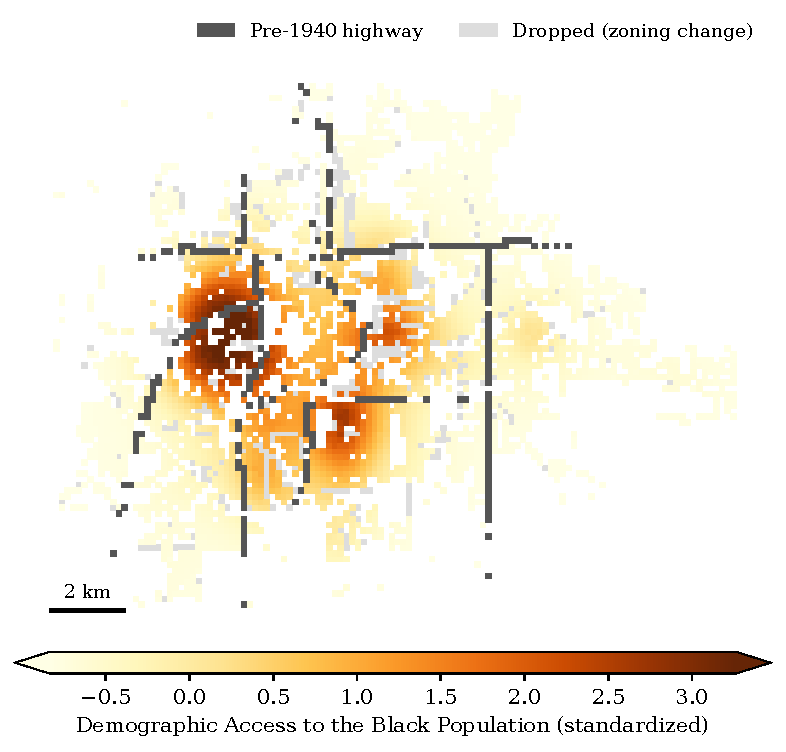
\includegraphics[width=\textwidth]{figures/dem_access_atlanta.pdf}
\par\vspace{0.5em}
\begin{minipage}{\textwidth}
\footnotesize Each square is a 150m grid cell in Atlanta, shaded by its distance-decayed access to the city's Black population (600m decay, 3km cutoff), standardized to mean zero and unit standard deviation within the city. The color scale is truncated at the 1st and 99th percentiles. Squares containing a highway built before 1940 are shown in dark gray; squares dropped from the sample because their zoning changed are shown in light gray.
\end{minipage}
\end{figure}
